\begin{figure}[ht]
    % \centering
    \begin{subfigure}[t]{.48\textwidth}
        % \centering
        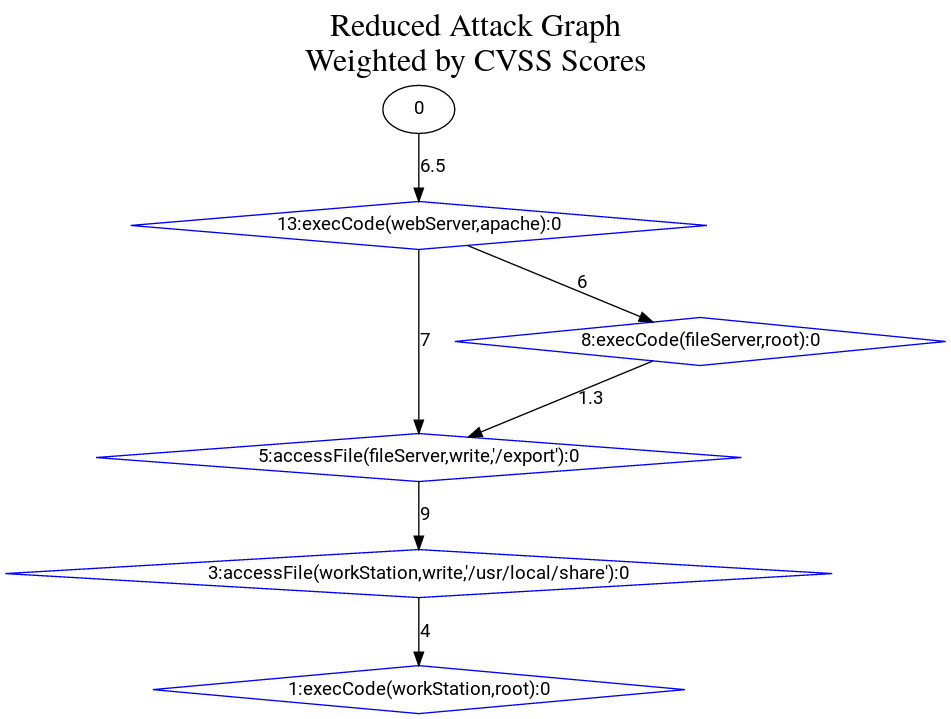
\includegraphics[width=\linewidth]{resource/img/ch_automation/from_ares_paper/ag_weight_mapped_time.png}
        \caption{}
        \label{fig:gm_002}
    \end{subfigure}
    \begin{subfigure}[t]{0.48\textwidth}
        % \centering
        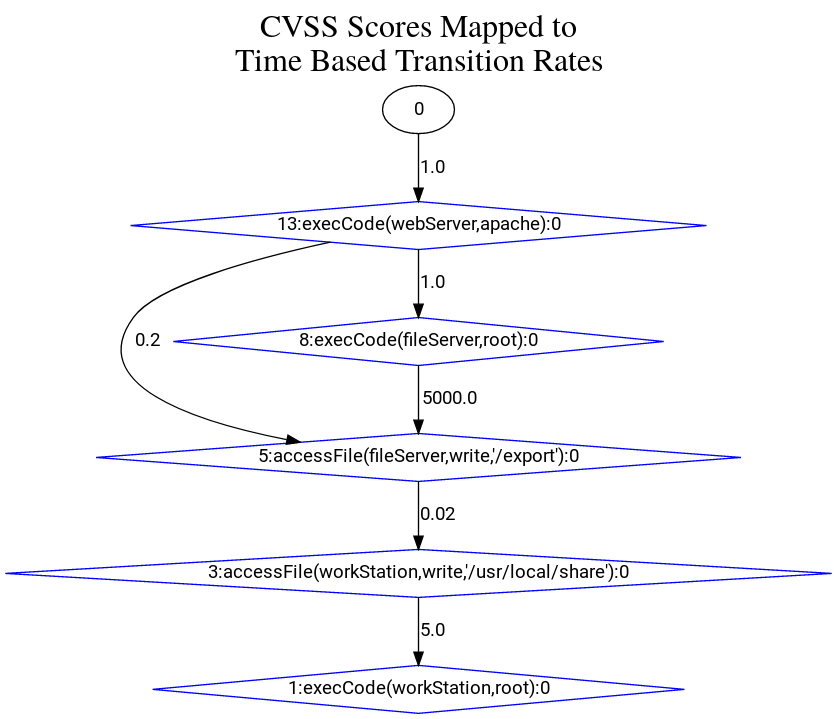
\includegraphics[width=\linewidth]{resource/img/ch_automation/from_ares_paper/map_time.png}
        \caption{} 
        \label{fig:gm_001}
    \end{subfigure}

    % \hfill
    \vspace{.2cm}
    \centering
    \begin{subfigure}[t]{0.48\textwidth}
        \centering
        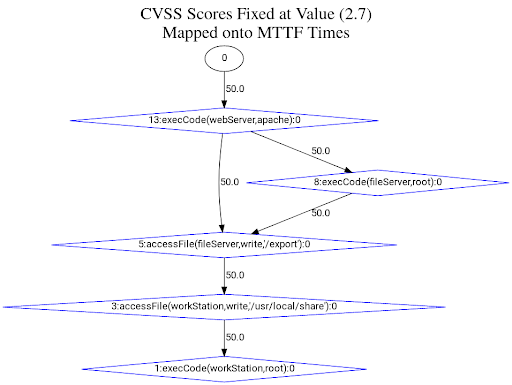
\includegraphics[width=\linewidth]{resource/img/ch_automation/from_ares_paper/map_fixed_time.png}
        \caption{} 
        \label{fig:gm_003}
    \end{subfigure}
    \begin{subfigure}[t]{0.48\textwidth}
        \centering
        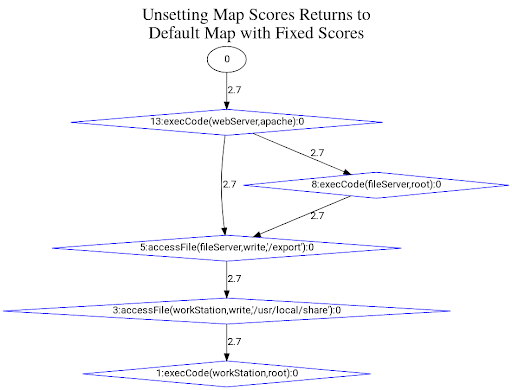
\includegraphics[width=\linewidth]{resource/img/ch_automation/from_ares_paper/map_fixed_unset.png}
        \caption{} 
        \label{fig:gm_004}
    \end{subfigure}
    \hfill
    \caption{Graph Weight Manipulation: These pairs should have equivalent security for the respective target metrics.}
    \label{fig:automation:mapGraph}
\end{figure}